\documentclass[10pt]{beamer}
\usetheme[
%%% option passed to the outer theme
%    progressstyle=fixedCircCnt,   % fixedCircCnt, movingCircCnt (moving is deault)
  ]{Feather}
  
% If you want to change the colors of the various elements in the theme, edit and uncomment the following lines

% Change the bar colors:
%\setbeamercolor{Feather}{fg=red!20,bg=red}

% Change the color of the structural elements:
%\setbeamercolor{structure}{fg=red}

% Change the frame title text color:
%\setbeamercolor{frametitle}{fg=blue}

% Change the normal text color background:
%\setbeamercolor{normal text}{fg=black,bg=gray!10}

%-------------------------------------------------------
% INCLUDE PACKAGES
%-------------------------------------------------------

\usepackage[utf8]{inputenc}
\usepackage[english]{babel}
\usepackage[T1]{fontenc}
\usepackage{helvet}

%-------------------------------------------------------
% DEFFINING AND REDEFINING COMMANDS
%-------------------------------------------------------

% colored hyperlinks
\newcommand{\chref}[2]{
  \href{#1}{{\usebeamercolor[bg]{Feather}#2}}
}

%-------------------------------------------------------
% INFORMATION IN THE TITLE PAGE
%-------------------------------------------------------

\title[] % [] is optional - is placed on the bottom of the sidebar on every slide
{ % is placed on the title page
      \textbf{Ticketfreier \"OPNV \& Sousveillance}
}

\subtitle[Ticketfreier \"OPNV \& Sousveillance]
{
      \textbf{Wie kann Gegenüberwachung helfen, um Ticketfreien ÖPNV zu erkämpfen?}
}

\author[Ticketfrei Kollektiv]
{      Ticketfrei Kollektiv \\
      {}
}

\institute[]
{
      Netzwerk für kybernetischen Anarchismus \& Sousveillance
  
  %there must be an empty line above this line - otherwise some unwanted space is added between the university and the country (I do not know why;( )
}

\date{\today}

%-------------------------------------------------------
% THE BODY OF THE PRESENTATION
%-------------------------------------------------------

\begin{document}

%-------------------------------------------------------
% THE TITLEPAGE
%-------------------------------------------------------

{\1% % this is the name of the PDF file for the background



\begin{frame}{Ticketfreier \"OPNV \& Sousveillance}{}

\maketitle
\tableofcontents

\end{frame}

\begin{frame}{Überblick}{}

\tableofcontents

\end{frame}

%-------------------------------------------------------
\section{ÖPNV}
%-------------------------------------------------------
\subsection{Unsere politischen Ziele}
\begin{frame}{Ticketfreier ÖPNV}{Infrastruktur für alle}
%-------------------------------------------------------

  \begin{itemize}
    \item<1-> Busse und Bahnen, komplett Steuer- oder Umlagenfinanziert
    \item<1-> Kosten für die Allgemeinheit sparen:
    \begin{itemize}
    	\item<1-> keine Automaten, keine Wartungskosten
    	\item<1-> keine Kontrolleure
    	\item<1-> weniger Verwaltungskosten
    	\item<1-> keine privatisierten Gewinne aus öffentlicher Infrastruktur/natürlichem Monopol
    \end{itemize}
    \item<2-> Weniger komplexes Ticketsystem
    \begin{itemize}
    	\item<1-> vor allem gut für Touristen/Zugezogene
    	\item<1-> vor allem, wenn man kein Deutsch spricht
    \end{itemize}
    \item<3-> Weniger Autofahrer
    \begin{itemize}
    	\item<1-> wenn die Autofahrer eh mitzahlen, kein Grund mehr Auto zu fahren
    	\item<1-> Gut für die Umwelt
    	\item<1-> weniger Smog, Lärm, Hektik, Verkehrsunfälle
    	\item<1-> weniger Verkehrschaos und Parkplatzsuche
    	\item<1-> Bäume statt Parkplätze
    	\item<1-> weniger Autokult
    \end{itemize}
  	\item<4-> Infrastruktur ist besser, je mehr Leute sie nutzen
  \end{itemize}
\end{frame}

\begin{frame}{Ticketfreier ÖPNV}{Demokratische Infrastruktur}

\begin{itemize}
    \item<1-> Barrieren für Nutzung sind das eine; Mitbestimmung das andere
    \item<1-> Infrastruktur bestimmt unser aller Leben
    \item<1-> Demokratische Mitbestimmung von Infrastruktur statt privaten Monopolen
	\item<1-> Wird allerdings nicht von Ticketfrei erreicht, sondern ist eher ein Ausblick, siehe Freifunk
\end{itemize}
    

\end{frame}


%-------------------------------------------------------
\section{Ticketfrei}
%-------------------------------------------------------
\subsection{Wie benutzt man Ticketfrei?}
\begin{frame}{Der Ticketfrei-Bot}{Wie benutzt man Ticketfrei}
%-------------------------------------------------------

\begin{block}{Kann ich grade schwarzfahren?}
  \begin{itemize}
    \item Auf https://twitter.com/nbg\_ticketfrei nachschauen, ob Kontrolleure gesehen wurden
    \item Mail Notifications - Mailingliste subscriben, und man kriegt immer ne Mail, wenn Kontrolleure gesehen wurden
  \end{itemize}
\end{block}

\begin{block}{Wenn man Kontrolleure sieht, kann man das auf drei Wegen melden:}
  \begin{itemize}
    \item Eine Mail an nbg\_ticketfrei@lists.links-tech.org
    \item Ein Tweet an @nbg\_ticketfrei
    \item Ein Toot an https://chaos.social/@nbg\_ticketfrei
  \end{itemize}
\end{block}

\begin{itemize}
    \item<2-> Die Nachricht muss mindestens 1 Wort wie "Konti, Bahn, Bus" etc. enthalten.
    \item<2-> Eigentlich ist Ticketfrei einfach nur ein Bot, der retweetet, was man ihm zu fressen gibt.
\end{itemize}

\end{frame}

%-------------------------------------------------------
\subsection{Schwachstellen von Ticketfrei}
\begin{frame}{Der Ticketfrei-Bot}{Schwachstellen von Ticketfrei}
%-------------------------------------------------------

\begin{block}{Funktioniert nur dann wirklich gut, wenn eine kritische Masse mitmacht}
  \begin{itemize}
    \item Aber übt auch bei weniger Leuten schon politischen Druck aus
  \end{itemize}
\end{block}

\begin{block}{Kann natürlich auch missbraucht werden für andere Themen}
  \begin{itemize}
    \item Muss man evtl Leute blocken, muss manuell maintained werden
  \end{itemize}
\end{block}

\begin{block}{Falschmeldungen sind unmöglich zu überprüfen}
  \begin{itemize}
    \item richten aber eigentlich auch keinen Schaden an
  \end{itemize}
\end{block}

\textbf{Weitere Anregungen?}

\end{frame}

%-------------------------------------------------------
\subsection{Die Idee}
\begin{frame}{Der Ticketfrei-Bot}{Wie ist Ticketfrei entstanden?}
%-------------------------------------------------------

\begin{itemize}
    \item<1-> Wir haben das in Berlin \& Hamburg funktionieren sehen und wollten das auch, aber der Code von denen war nicht open source
    \item<1-> Ein Team von 2 Leuten haben sich mal nen Tag hingesetzt, und den Großteil programmiert.
    \item<1-> Später wurde noch etwas verfeinert.
    \item<2-> Der ganze Bot ist auf Github: \url{https://github.com/ticketfrei/ticketfrei/}
  \begin{itemize}
    \item Dadurch kann der Code nicht nur von jedem genutzt, sondern auch verändert werden.
  \end{itemize}
    \item<2-> Wurde von Laien geschrieben, und hat nicht viel Kenntnisse/Arbeit erfordert - jede*r kann programmieren!
	\item<2-> Und jede*r sollte programmieren - man kann einiges mit Code erreichen.
  \begin{itemize}
    \item vor allem nicht nur cis-dudes :P
  \end{itemize}
\end{itemize}
    

\end{frame}

%-------------------------------------------------------
\subsection{Architektur des Bots}
\begin{frame}{Der Ticketfrei-Bot}{Die Architektur}
%-------------------------------------------------------

\begin{block}{{\tt retweetbot.py, retootbot.py, mailbot.py}}
  \begin{itemize}
    \item hören auf neue Meldungen (Mentions auf Twitter/Mastodon, Mails)
    \item verbreiten die Meldungen weiter (Retweets, Boosts, Rundmails)
    \item Können jeweils auch einzeln gestartet werden
  \end{itemize}
\end{block}

\begin{block}{{\tt ticketfrei.py}}
  \begin{itemize}
    \item Damit kann man alle Bots zusammen ausführen und miteinander reden lassen
  \end{itemize}
\end{block}

\begin{block}{{\tt config.toml}}
  \begin{itemize}
    \item Eine zentrale Konfigurationsdatei, um Einstellungen einfach setzen zu können
  \end{itemize}
\end{block}

\end{frame}
%-------------------------------------------------------
\begin{frame}{Der Ticketfrei-Bot}{Die Architektur}

\begin{block}{{\tt trigger.py}}
  \begin{itemize}
    \item eine python-Klasse, die darauf achtet, ob Wörter im Report in der White- oder Blacklist sind:
    \item mindestens 1 Wort wie "Konti, Bahn, Bus" muss enthalten sein
    \item gewisse antisemitische, sexistische, homophobe, rassistische Beleidigungen sind geblacklistet
  \end{itemize}
\end{block}

\begin{block}{{\tt logger.py}}
  \begin{itemize}
    \item Kümmert sich darum, dass Errors geloggt werden, stellt Crash Reports zusammen
  \end{itemize}
\end{block}

\begin{block}{{\tt sendmail.py}}
  \begin{itemize}
    \item Versendet alle Mails, zB wenn der Bot crasht
  \end{itemize}
\end{block}

\end{frame}

%-------------------------------------------------------
\subsection{Entwicklungs-Roadmap}
\begin{frame}{Der Ticketfrei-Bot}{Wo wollen wir hin?}
%-------------------------------------------------------

\begin{itemize}
  \item<1-> Es soll auch für Leute in anderen Städten einfacher werden, sich Ticketfrei für ihre Stadt zu installieren
  \item<1-> Mit einem Webinterface könnten Leute sich das mit ein paar Knopfdrücken installieren, ohne auf die Kommandozeile zu müssen oder einen Server zu brauchen
  \item<2-> Dann können sie sich auf die Promotion-Arbeit konzentrieren, statt aufs technische
  \item<2-> Im Github-Repository gibt es auch Vorlagen für Promotion-Material, das man anpassen kann: \url{https://github.com/ticketfrei/promotion}
  \item<2-> Die Website wird unter \url{https://ticketfrei.links-tech.org} verfügbar sein.
\end{itemize}

\end{frame}

\begin{frame}
	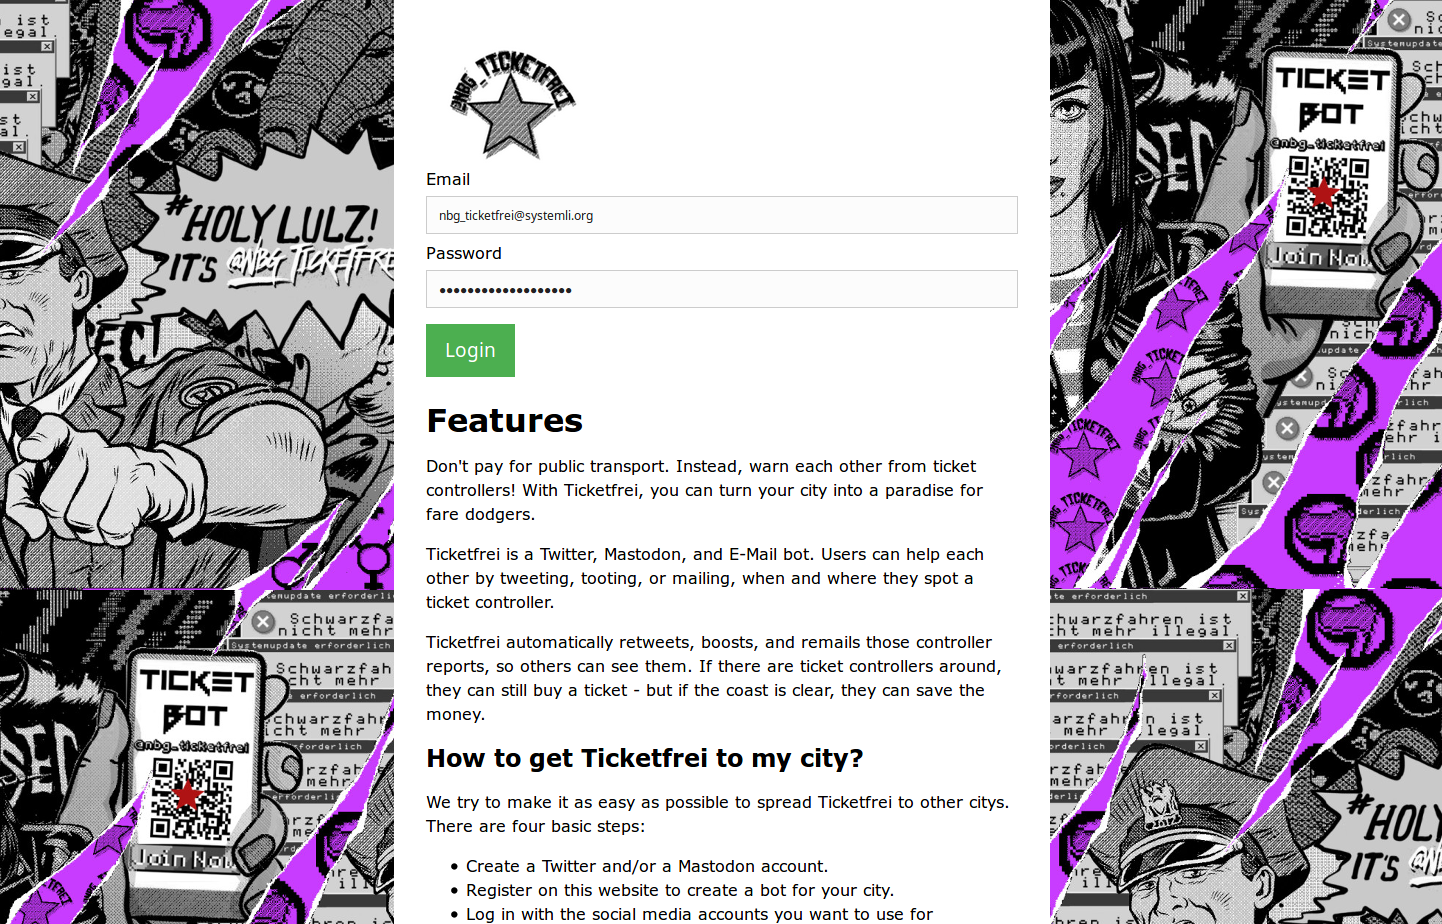
\includegraphics[width=\textwidth]{screenshots/Screenshot_2018-03-30_01-22-59.png}	
\end{frame}
\begin{frame}
	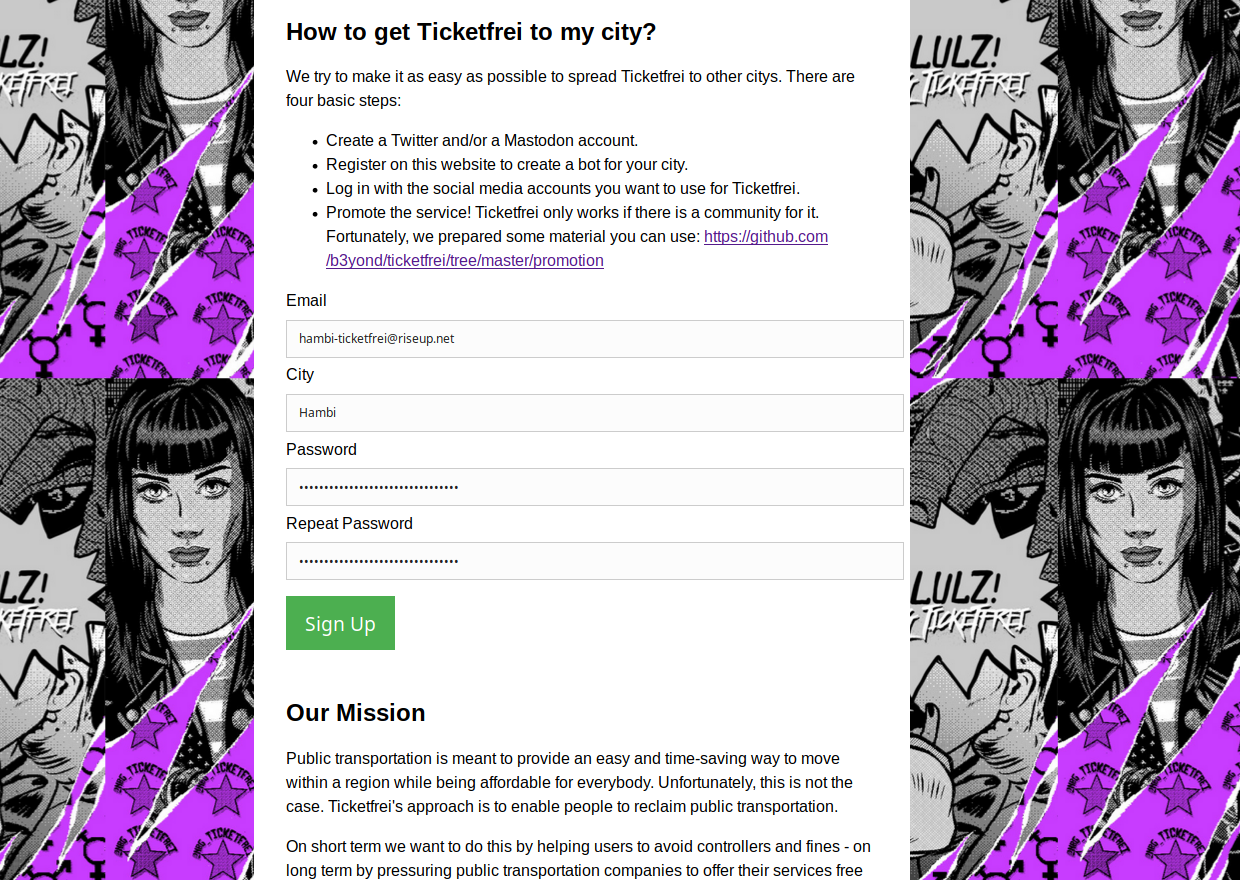
\includegraphics[width=\textwidth]{screenshots/Screenshot_2018-03-30_01-10-40.png}	
\end{frame}
\begin{frame}
	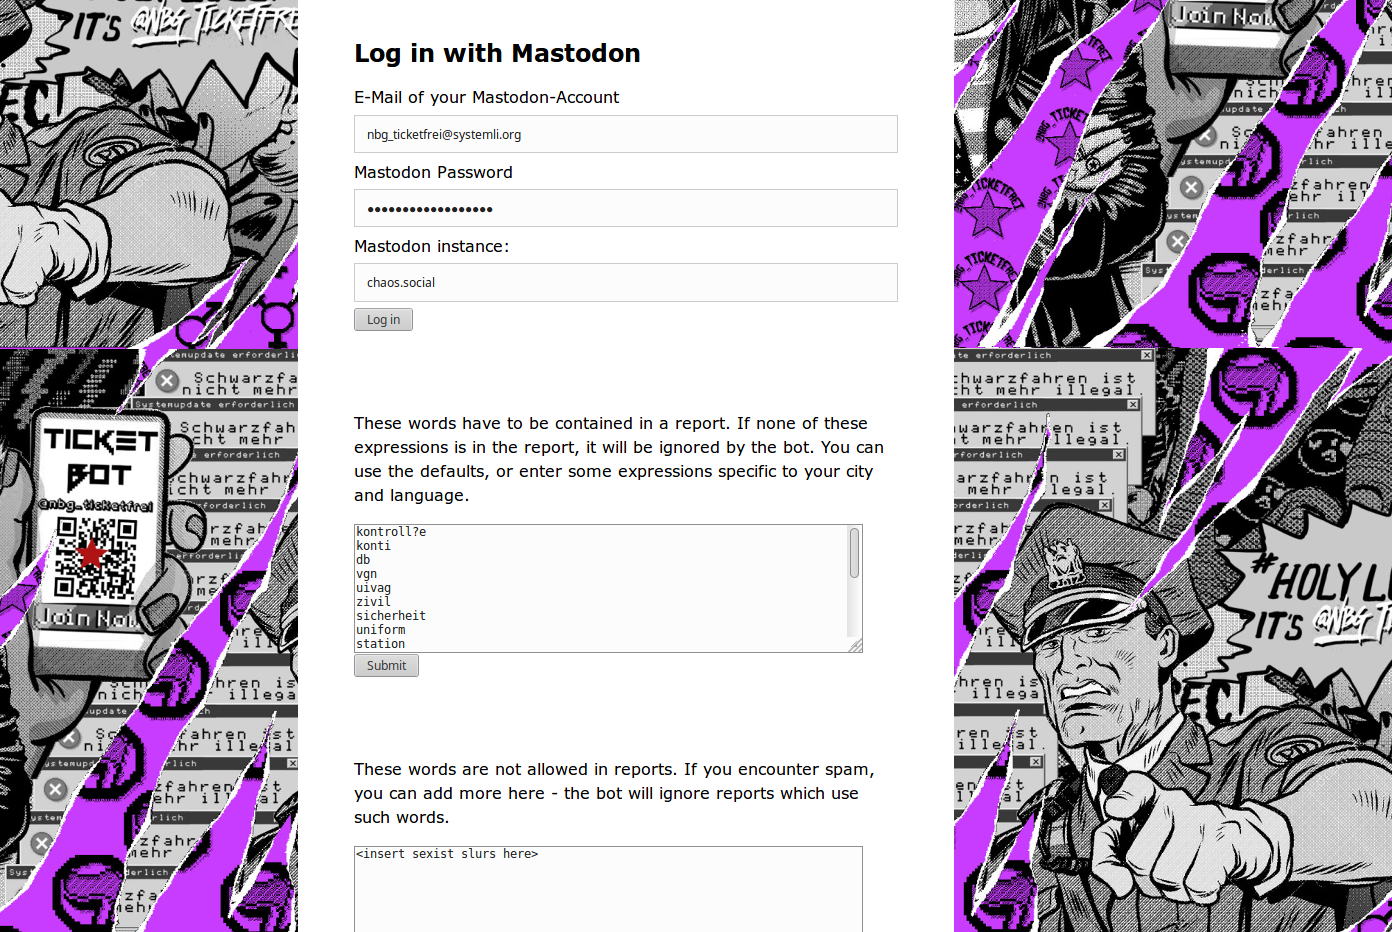
\includegraphics[width=\textwidth]{screenshots/Screenshot_2018-03-30_01-13-16.png}	
\end{frame}


\subsection{Step-by-Step}
\begin{frame}{The Ticketfrei Bot}{Step-by-Step}

\begin{itemize}
  \item Create an Account at https://ticketfrei.links-tech.org:
  \begin{itemize}
    \item E-Mail-Adress, City, Password
  \end{itemize}
  \item Add Social-Media accounts to your Ticketfrei account
  \item Change the text on https://ticketfrei.links-tech.org/city/Nürnberg
  \item Promote the use of the bot in your city
\end{itemize}

\end{frame}
\begin{frame}{The Ticketfrei Bot}{Step-by-Step}

\begin{block}{{Add Twitter}}
  \begin{itemize}
    \item Register a twitter account
    \item Click on "Login with Twitter" in the settings
    \item Log in to the twitter account of the bot
    \item Authorize the Ticketfrei app
  \end{itemize}
\end{block}

\end{frame}
\begin{frame}{The Ticketfrei Bot}{Step-by-Step}

\begin{block}{{Add Mastodon}}
  \begin{itemize}
    \item Register a mastodon account
    \item Enter the account's e-mail address, the password, and the mastodon server to the settings
    \item Click on "Log in"
  \end{itemize}
\end{block}

\end{frame}
\begin{frame}{The Ticketfrei Bot}{Step-by-Step}

\begin{block}{{Add Telegram}}
  \begin{itemize}
    \item Write to @botfather on Telegram to register a Telegram Bot
    \item Enter the API key which @botfather gives to you into the settings
    \item Click on "Login with Telegram"
  \end{itemize}
\end{block}

\end{frame}

\subsection{promotion}
\begin{frame}{The Ticketfrei Bot}{Promotion}

\begin{itemize}
  \item Leaflets in the local leftist scene, with more radical message
  \item Leaflets for the public, which explains goals and talks about the environment, but also explains the bot
  \item Example Leaflets are available in the GitHub-Repository at \url{https://github.com/ticketfrei/promotion}
  \item<2-> Aktionsschwarzfahren is a good way to both spread leaflets and dodge the fare legally
  \item<3-> With enough public attention you can try to start a referendum or bring the topics to political parties for policy making
  \item<4-> Studies about the practicability and cost effectiveness of ticket-free public transport in your area are also useful
\end{itemize}

\end{frame}

%-------------------------------------------------------
\section{Sousveillance}
\subsection{Kybernetik und Überwachung}
\begin{frame}{Surveillance vs. Sousveillance}{1. Surveillance / Überwachung}
%-------------------------------------------------------

\begin{itemize}
  \item<1-> Kybernetik/Maxwellscher Demon: mit genug Daten ist alles berechenbar?
  \begin{itemize}
    \item<2-> Ob das wirklich funktioniert, spielt keine Rolle
    \item<2-> These: Um zu beweisen, dass das nicht funktionieren kann, bräuchte man mehr Daten als die Überwacher
  \end{itemize}
  \item<3-> Kybernetik kommt von lat. Kybernetes: Steuermann, Governor. Mit Herrschaft assoziiert
  \item<3-> So viele Daten wie möglich sammeln, um sie verknüpfen zu können
  \item<3-> Geheimhaltung der Daten, um Wissensvorsprung gegenüber anderen Parteien zu haben
  \item<4-> Wird erst gefährlich, wenn die Überwachenden auch Gewalt ausüben können
  \item<4-> Man weiß eigentlich nie, welche Daten andere über einen haben, deswegen schwer sich dagegen zu schützen
\end{itemize}

\end{frame}

%-------------------------------------------------------
\subsection{Definition Sousveillance}
\begin{frame}{Surveillance vs. Sousveillance}{2. Sousveillance / Unterwachung}
%-------------------------------------------------------

\begin{itemize}
  \item<1-> Definition Sousveillance:
  \begin{itemize}
    \item Überwachung von unten nach oben -> Ziel ist mächtiger als man selbst
    \item Veröffentlichung der Ergebnisse
  \end{itemize}
  \item<2-> Auch auf Geheimdienste und Polizei hat Beobachtung disziplinierende Wirkung
  \begin{itemize}
    \item<2-> Müssen auf andere Strategien ausweichen, Höhere Kosten
  \end{itemize}
  \item<2-> Geheimhaltung ist immer schwieriger/teurer als Veröffentlichung
\end{itemize}

\end{frame}

%-------------------------------------------------------
\subsection{Beispiele für Sousveillance}
\begin{frame}{Surveillance vs. Sousveillance}{Beispiele für Sousveillance}
%-------------------------------------------------------

\begin{itemize}
  \item<1-> Whistleblower: Chelsea Manning, Edward Snowden, und WikiLeaks
  \item<1-> (Investigativ-)Journalismus: Was macht denn der Staat eig so?
  \begin{itemize}
    \item<2-> Panama Papers, Paradise Papers
  \end{itemize}
  \item<2-> Bei (Demos etc.) Polizeieinsätze (-gewalt) filmen
  \begin{itemize}
    \item<2-> den größten Zulauf hatte OccupyWallstreet, nachdem Videos von Polizeigewalt auftauchten
    \item<2-> Das Drama an der Berufsschule war auch deswegen so groß in den Medien, weil die Polizei so eskaliert ist
  \end{itemize}
  \item<3-> Ticketfrei: Wo sind gerade Ticketkontrolleure?
\end{itemize}

\end{frame}


%-------------------------------------------------------
\subsection{Fazit}
\begin{frame}{Surveillance vs. Sousveillance}{Fazit}
%-------------------------------------------------------

\text Die Überwachung lässt sich nicht mehr zurückdrehen, und das ist politisch auch nicht gewollt.
Das Privateigentum will durch ständige Kontrolle aufrechterhalten werden, ökonomische und
politische Teilhabe soll verhindert werden. Überwachung hilft dabei und entwickelt sich zu
ganz neuen Geschäftsmodellen.

\text \break

\text Also müssen wir uns wehren, und selbst Gegenüberwachen, um uns vor den Mächtigen zu schützen.
Sousveillance ist ein gutes Mittel gegen die Kontrolleursgesellschaft.

\end{frame}


{\1
\begin{frame}[plain,noframenumbering]
	\finalpage{Danke fürs Zuhören!}
\end{frame}}

\end{document}
